
\documentclass[letterpaper,hide notes,xcolor={table,svgnames},pdftex,10pt]{beamer}
\def\showexamples{t}

\usecolortheme{crane}
\setbeamertemplate{navigation symbols}{}

\usetheme{MyPittsburgh}
\usepackage{hyperref}
\usepackage{graphicx,xspace}
\usepackage[normalem]{ulem}
\usepackage{multicol}
\usepackage{amsmath,amssymb,amsthm,graphicx,xspace}
\newcommand\SF[1]{$\bigstar$\footnote{SF: #1}}

\usepackage[sfdefault,lf]{carlito}
\usepackage[T1]{fontenc}
\usepackage[scaled]{beramono}
\usepackage{tikzpagenodes}
\newcommand{\Rplus}{\protect\hspace{-.1em}\protect\raisebox{.35ex}{\small{\small\textbf{+}}}}
\newcommand{\Cpp}{\mbox{C\Rplus\Rplus}\xspace}

\newcounter{tmpnumSlide}
\newcounter{tmpnumNote}

\newcommand\mnote[1]{%
	\addtocounter{tmpnumSlide}{1}
	\ifdefined\showcues {~\tiny\fbox{\arabic{tmpnumSlide}}}\fi
	\note{\setlength{\parskip}{1ex}\addtocounter{tmpnumNote}{1}\textbf{\Large \arabic{tmpnumNote}:} {#1\par}}}

\newcommand\mmnote[1]{\note{\setlength{\parskip}{1ex}#1\par}}


\newcommand\mquestion[2]{{~\color{red}\fbox{?}}\note{\setlength{\parskip}{1ex}\par{\Large \textbf{?}} #1} \note{\setlength{\parskip}{1ex}\par{\Large \textbf{A}} #2\par}\ifdefined \presentationonly \pause \fi}

\newcommand\blackboard[1]{%
	\ifdefined   \showblackboard
		{#1}
	\else {\begin{center} \fbox{\colorbox{blue!30}{%
						\begin{minipage}{.95\linewidth}%
							\hspace{\stretch{1}} Some space intentionally left blank; done at the blackboard.%
						\end{minipage}}}\end{center}}%
	\fi%
}

\usepackage{listings}
\lstset{%
	keywordstyle=\bfseries,
	aboveskip=15pt,
	belowskip=15pt,
	captionpos=b,
	identifierstyle=\ttfamily,
	frame=lines,
	numbers=left, basicstyle=\scriptsize, numberstyle=\tiny, stepnumber=0, numbersep=2pt}

\usepackage{siunitx}
\newcommand\sius[1]{\num[group-separator = {,}]{#1}\si{\micro\second}}
\newcommand\sims[1]{\num[group-separator = {,}]{#1}\si{\milli\second}}
\newcommand\sins[1]{\num[group-separator = {,}]{#1}\si{\nano\second}}
\sisetup{group-separator = {,}, group-digits = true}

%% -------------------- tikz --------------------
\usepackage{tikz}
\usetikzlibrary{positioning}
\usetikzlibrary{arrows,backgrounds,automata,decorations.shapes,decorations.pathmorphing,decorations.markings,decorations.text}

\tikzstyle{place}=[circle,draw=blue!50,fill=blue!20,thick, inner sep=0pt,minimum size=6mm]
\tikzstyle{transition}=[rectangle,draw=black!50,fill=black!20,thick, inner sep=0pt,minimum size=4mm]

\tikzstyle{block}=[rectangle,draw=black, thick, inner sep=5pt]
\tikzstyle{bullet}=[circle,draw=black, fill=black, thin, inner sep=2pt]

\tikzstyle{pre}=[<-,shorten <=1pt,>=stealth',semithick]
\tikzstyle{post}=[->,shorten >=1pt,>=stealth',semithick]
\tikzstyle{bi}=[<->,shorten >=1pt,shorten <=1pt, >=stealth',semithick]

\tikzstyle{mut}=[-,>=stealth',semithick]

\tikzstyle{treereset}=[dashed,->, shorten >=1pt,>=stealth',thin]

\usepackage{ifmtarg}
\usepackage{xifthen}
\makeatletter
% new counter to now which frame it is within the sequence
\newcounter{multiframecounter}
% initialize buffer for previously used frame title
\gdef\lastframetitle{\textit{undefined}}
% new environment for a multi-frame
\newenvironment{multiframe}[1][]{%
	\ifthenelse{\isempty{#1}}{%
		% if no frame title was set via optional parameter,
		% only increase sequence counter by 1
		\addtocounter{multiframecounter}{1}%
	}{%
		% new frame title has been provided, thus
		% reset sequence counter to 1 and buffer frame title for later use
		\setcounter{multiframecounter}{1}%
		\gdef\lastframetitle{#1}%
	}%
	% start conventional frame environment and
	% automatically set frame title followed by sequence counter
	\begin{frame}%
		\frametitle{\lastframetitle~{\normalfont(\arabic{multiframecounter})}}%
		}{%
	\end{frame}%
}
\makeatother

\makeatletter
\newdimen\tu@tmpa%
\newdimen\ydiffl%
\newdimen\xdiffl%
\newcommand\ydiff[2]{%
	\coordinate (tmpnamea) at (#1);%
	\coordinate (tmpnameb) at (#2);%
	\pgfextracty{\tu@tmpa}{\pgfpointanchor{tmpnamea}{center}}%
	\pgfextracty{\ydiffl}{\pgfpointanchor{tmpnameb}{center}}%
	\advance\ydiffl by -\tu@tmpa%
}
\newcommand\xdiff[2]{%
	\coordinate (tmpnamea) at (#1);%
	\coordinate (tmpnameb) at (#2);%
	\pgfextractx{\tu@tmpa}{\pgfpointanchor{tmpnamea}{center}}%
	\pgfextractx{\xdiffl}{\pgfpointanchor{tmpnameb}{center}}%
	\advance\xdiffl by -\tu@tmpa%
}
\makeatother
\newcommand{\copyrightbox}[3][r]{%
	\begin{tikzpicture}%
		\node[inner sep=0pt,minimum size=2em](ciimage){#2};
		\usefont{OT1}{phv}{n}{n}\fontsize{4}{4}\selectfont
		\ydiff{ciimage.south}{ciimage.north}
		\xdiff{ciimage.west}{ciimage.east}
		\ifthenelse{\equal{#1}{r}}{%
			\node[inner sep=0pt,right=1ex of ciimage.south east,anchor=north west,rotate=90]%
			{\raggedleft\color{black!50}\parbox{\the\ydiffl}{\raggedright{}#3}};%
		}{%
			\ifthenelse{\equal{#1}{l}}{%
				\node[inner sep=0pt,right=1ex of ciimage.south west,anchor=south west,rotate=90]%
				{\raggedleft\color{black!50}\parbox{\the\ydiffl}{\raggedright{}#3}};%
			}{%
				\node[inner sep=0pt,below=1ex of ciimage.south west,anchor=north west]%
				{\raggedleft\color{black!50}\parbox{\the\xdiffl}{\raggedright{}#3}};%
			}
		}
	\end{tikzpicture}
}


%% --------------------

%\usepackage[excludeor]{everyhook}
%\PushPreHook{par}{\setbox0=\lastbox\llap{MUH}}\box0}

%\vspace*{\stretch{1}

%\setbox0=\lastbox \llap{\textbullet\enskip}\box0}

\setlength{\parskip}{\fill}

\newcommand\noskips{\setlength{\parskip}{1ex}}
\newcommand\doskips{\setlength{\parskip}{\fill}}

\newcommand\xx{\par\vspace*{\stretch{1}}\par}
\newcommand\xxs{\par\vspace*{2ex}\par}
\newcommand\tuple[1]{\langle #1 \rangle}
\newcommand\code[1]{{\sf \footnotesize #1}}
\newcommand\ex[1]{\uline{Example:} \ifdefined \presentationonly \pause \fi
	\ifdefined\showexamples#1\xspace\else{\uline{\hspace*{2cm}}}\fi}

\newcommand\ceil[1]{\lceil #1 \rceil}


\AtBeginSection[]
{
	\begin{frame}
		\frametitle{Outline}
		\tableofcontents[currentsection]
	\end{frame}
}



\pgfdeclarelayer{edgelayer}
\pgfdeclarelayer{nodelayer}
\pgfsetlayers{edgelayer,nodelayer,main}

\tikzstyle{none}=[inner sep=0pt]
\tikzstyle{rn}=[circle,fill=Red,draw=Black,line width=0.8 pt]
\tikzstyle{gn}=[circle,fill=Lime,draw=Black,line width=0.8 pt]
\tikzstyle{yn}=[circle,fill=Yellow,draw=Black,line width=0.8 pt]
\tikzstyle{empty}=[circle,fill=White,draw=Black]
\tikzstyle{bw} = [rectangle, draw, fill=blue!20,
text width=4em, text centered, rounded corners, minimum height=2em]

\newcommand{\CcNote}[1]{% longname
	This work is licensed under the \textit{Creative Commons #1 3.0 License}.%
}
\newcommand{\CcImageBy}[1]{%
	\includegraphics[scale=#1]{creative_commons/cc_by_30.pdf}%
}
\newcommand{\CcImageSa}[1]{%
	\includegraphics[scale=#1]{creative_commons/cc_sa_30.pdf}%
}
\newcommand{\CcImageNc}[1]{%
	\includegraphics[scale=#1]{creative_commons/cc_nc_30.pdf}%
}
\newcommand{\CcGroupBySa}[2]{% zoom, gap
	\CcImageBy{#1}\hspace*{#2}\CcImageNc{#1}\hspace*{#2}\CcImageSa{#1}%
}
\newcommand{\CcLongnameByNcSa}{Attribution-NonCommercial-ShareAlike}

\newenvironment{changemargin}[1]{% 
	\begin{list}{}{% 
		\setlength{\topsep}{0pt}% 
		\setlength{\leftmargin}{#1}% 
		\setlength{\rightmargin}{1em}
		\setlength{\listparindent}{\parindent}% 
		\setlength{\itemindent}{\parindent}% 
		      \setlength{\parsep}{\parskip}% 
		      }% 
		\item[]}{\end{list}}




\title{Lecture 19 --- Deadlock Avoidance }

\author{Jeff Zarnett \\ \small \texttt{jzarnett@uwaterloo.ca}}
\institute{Department of Electrical and Computer Engineering \\
  University of Waterloo}
\date{\today}


\begin{document}

\begin{frame}
  \titlepage

 \end{frame}

\begin{frame}
\frametitle{Deadlock Avoidance}

We were attempting to rule deadlock out categorically by eliminating one of the three preconditions for deadlock to be possible. 

If successful, then we can be sure that deadlock does not occur. 

Unfortunately, eliminating the pillars came with some conditions and the best we could accomplish was merely making deadlock less likely. 

Thus, we are forced to live with a system where a deadlock is possible. 
\end{frame}


\begin{frame}
\frametitle{Deadlock Avoidance}

Deadlock being possible is not the same thing as deadlock being inevitable.

We can take steps to avoid it if there is a danger of it actually happening. 

The basic strategy is: do not allow a cycle in the resource allocation graph.


\end{frame}

\begin{frame}
\frametitle{Deadlocked Diners}

In the dining philosophers problem: limit the number of concurrently-eating philosophers to four, even though the table has five seats. 

With only four philosophers and five chopsticks, there were insufficient requests to complete a cycle. 

This solution is suitable, but not necessarily generalizable to all situations.

\end{frame}

\begin{frame}[fragile]
\frametitle{Ordering of Resources}

Impose ordering on resource requests. Recall this example:

\begin{multicols}{2}
\textbf{Thread P}
  \begin{verbatim}
	 1. wait( a ) 
	 2. wait( b )
	 3. [critical section]
	 4. signal( a )
	 5. signal( b )
  \end{verbatim}
\columnbreak
\textbf{Thread Q}
  \begin{verbatim}
	 1. wait( b ) 
	 2. wait( a )
	 3. [critical section]
	 4. signal( b )
	 5. signal( a )
  \end{verbatim}
\end{multicols}
\vspace{-2em}

Deadlock would not take place if both threads requested these two resources in the same order, whether \texttt{a} then \texttt{b} or \texttt{b} then \texttt{a}. 

\end{frame}

\begin{frame}
\frametitle{Ordering of Resources}

Let's generalize and formalize this principle.
 
The set of all resources in the system is $R = \{R_{0}, R_{1}, R_{2}, ... R_{m}\}$.

We assign to each resource $R_{k}$ a unique integer value. Let us define this function as $f(R_{i})$, that maps a resource to an integer value. 

This integer value is used to compare two resources: if a process has been assigned resource $R_{i}$, that process may request $R_{j}$ only if $f(R_{j}) > f(R_{i})$.


\end{frame}

\begin{frame}
\frametitle{Ordering of Resources}

Note that this is a strictly greater-than relationship. 

If the process needs more than one of $R_{i}$ then the request for all of these must be made at once (in a single request). 

To get $R_{i}$ when already in possession of a resource $R_{j}$ where $f(R_{j}) > f(R_{i})$, the process must release any resources $R_{k}$ where $f(R_{k}) \geq f(R_{i})$. 

If these two protocols are followed, then a circular-wait condition cannot hold.

\end{frame}

\begin{frame}
\frametitle{Ordering of Resources}

Back to the philosophers: we assign each chopstick a number from 0 to 5. 

Each philosopher must then request them in ascending order. 

The first philosopher requests 0, on her left, and then 1, on her right. 

The second requests chopstick 1 and then chopstick 2. 

This continues until the last philosopher who would previously have requested chopstick 4 and then 0, but under the new rules, this is forbidden. 

This philosopher must instead request 0 on his right, and then 4, on his left. 

This last philosopher will be blocked when trying to acquire chopstick 0 and it means chopstick 4 will be available for the second-to-last philosopher. 

Thus, deadlock is avoided.

\end{frame}

\begin{frame}
\frametitle{The Proof is the Proof}

Assume a circular wait is present. 

Let the set of processes in the circular wait be $\{P_{0}, P_{1}, ... P_{n}\}$ and the set of resources be $\{R_{0}, R_{1}, ... R_{n}\}$. 

The cycle is formed as: $P_{i}$ waits for resource $R_{i}$ and that resource is held by $P_{i+1}$. 

The exception is the case of $P_{n}$, which waits for resource $R_{n}$ that is held by $P_{0}$.

Since Process $P_{i+1}$ holds resource $R_{i}$ while requesting $R_{i+1}$, this means $f(R_{i}) < f(R_{i+1})$ for all $i$. 

But this means that $f(R_{0}) < f(R_{1}) < ... < f(R_{n}) < f(R_{0})$. 

It cannot be the case that $f(R_{0}) < f(R_{0})$: a contradiction.

\end{frame}

\begin{frame}
\frametitle{Ordering Resources}

In development this is usually enforced just by coding convention and code review. 

If you say that mutexes must always be acquired in alphabetical order (or their order in some file), if everyone sticks to that there will be no issue.

But may not be as easy as that in a real-world scenario...

\end{frame}

\begin{frame}
\frametitle{Stay Alert, Stay Safe}

Alternative: each process will need to give the operating system some additional information about what resources might be requested. 

Processes need to say in advance of execution what is the maximum number of resources of each type they might conceivably need. 

Perhaps process $A$ needs the tape drive first, then the printer, and process $B$ needs the printer and then the tape drive. 

With this knowledge, the system can make more intelligent decisions about when to run a process or make it wait, to avoid getting into a deadlock.

\end{frame}



\begin{frame}
\frametitle{Safe States}


We say a state is \alert{safe} if there is some scheduling order in which every process can run to completion.

Even if all of them suddenly request their maximum resources immediately. 

Hence why we needed to know in advance the maximum resources that could be required by the process. 

\end{frame}

\begin{frame}
\frametitle{Safe Sequences}

More formally, there must exist a \alert{safe sequence}.

A sequence of processes $<P_{1}, P_{2}, ... P_{n}$ is a safe sequence in the current allocation state if:

For each $P_{i}$ the resource requests that $P_{i}$ can still make can be satisfied by the currently available resources plus resources held by $P_{j}$ where $j < i$. 

If a resource $P_{i}$ needs is not currently available, $P_{i}$ can wait until all $P_{j}$ have finished and releases its resources. 

When $P_{i}$ terminates, $P_{i+1}$ can obtain its needed resources and continue.

\end{frame}

\begin{frame}
\frametitle{Safe/Unsafe}

Any state that is not safe is considered \alert{unsafe}. 

If the system is in a safe state, then there is no deadlock. 

Being in an unsafe state does not mean that there is a deadlock, but it means a deadlock is possible. 

The analysis we do is the worst case scenario: every process immediately requests the maximum resources it could ever use. 

Perhaps the processes do not make those requests in reality.

\end{frame}

\begin{frame}
\frametitle{Safe State Example}

There are three processes $A$, $B$, and $C$. 

Assume there is only one resource, and a maximum of 10 instances exist. 

Suppose $A$ has 3 resources but may request up to 9.\\
$B$ has 2 and may request up to 4.\\
$C$ has 2 and may request up to 7. 

There are 3 resources currently free.

\begin{center}
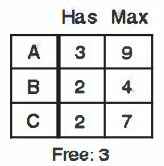
\includegraphics[width=0.25\textwidth]{images/safe-state-initial.png}
\end{center}

\end{frame}

\begin{frame}
\frametitle{Being Safe}


For a state to be safe, we need one path that allows all processes to complete. 

Multiple solutions may exist, and there may be paths that lead to deadlock. 

\begin{center}
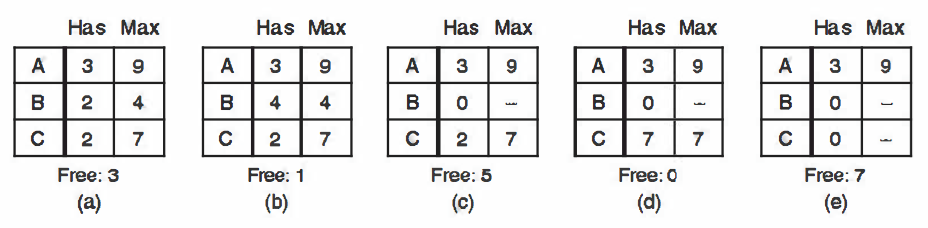
\includegraphics[width=0.9\textwidth]{images/safe-state.png}
\end{center}


\end{frame}

\begin{frame}
\frametitle{Crossing the Line}

Suppose, however, $A$ requests and gets another resource. 

In that case, the initial condition has changed so that $A$ has 4 resources and there are 2 free resources. 

Or, in the diagram below, the state changes from (a) to (b).

\begin{center}
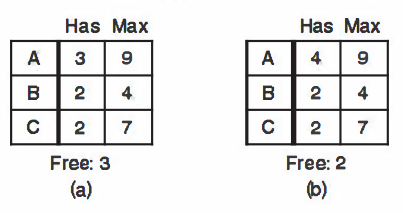
\includegraphics[width=0.5\textwidth]{images/unsafe-state-initial.png}
\end{center}


\end{frame}

\begin{frame}
\frametitle{Evaluating the New Initial State}

Trying to find a way for all processes to complete is not possible.

Thus, this state is unsafe.

This does not mean that deadlock is present or certain. 

The analysis is worst-case.

\end{frame}

\begin{frame}
\frametitle{Resource-Allocation-Graph Algorithm}

The fourth condition for deadlock is modelled, typically as being a resource allocation graph with a cycle in it. 

Idea: let us use that idea to avoid deadlock by having the operating system maintain a resource allocation graph. 

This works if there is only one instance of each resource and still requires that all the resources that a process will require must be declared in advance. 

This condition does not have to be strictly adhered to if the system allows additional requests only when no requests have yet been granted.

\end{frame}

\begin{frame}
\frametitle{Resource-Allocation-Graph}

The model for resource allocation graphs earlier had two kinds of edges:

One representing requests (a process requests a resource); and
One representing allocation (a resource currently belongs to a process). 

We will require a new type of edge in the graph: a \alert{claim} edge. 

When the process actually makes the request for the resource, a claim edge is converted to a request edge. 

Upon release the assignment edge reverts to a claim edge.
\end{frame}

\begin{frame}
\frametitle{Resource Allocation Graph}

\begin{center}
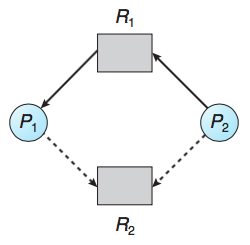
\includegraphics[width=0.3\textwidth]{images/resource-allocation-graph-claim.png}
\end{center}

A resource request will only be granted if converting the request edge to an assignment edge will not result in a cycle in the graph.

If no cycle is found, then allocation of the resource will not move the system into an unsafe state. 

If a cycle is found, the request should not be granted, as it risks a deadlock.

\end{frame}

\begin{frame}
\frametitle{The Banker's Algorithm}

The previous algorithm is applicable only if all resource requests are known in advance and there is only one instance of each resource.

The banker's algorithm is more general: it allows for resources with multiple instances. 

It received this name because it is hypothetically an algorithm that a small town banker might follow.

He or she is trying to prevent allocating the cash on hand in such away that he or she could no longer satisfy customers.

\end{frame}

\begin{frame}
\frametitle{The Banker's Algorithm}


The analysis we did earlier to determine if a state is safe or unsafe, is the foundation of the banker's algorithm. 

\begin{center}
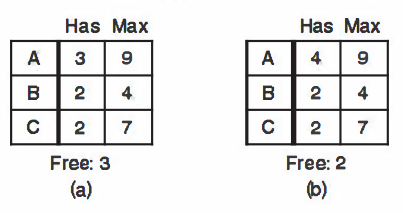
\includegraphics[width=0.35\textwidth]{images/unsafe-state-initial.png}
\end{center}

Granting the request from process $A$ moved the system safe to unsafe.

The operating system, when it receives a resource request, will evaluate the new state to see if it would transition the system to an unsafe state.

\end{frame}

\begin{frame}
\frametitle{The Banker's Algorithm}

If so, the request will be denied or $A$ will be blocked until the request can be fulfilled without putting the system in an unsafe state. 

Holding to this condition means deadlock will be avoided.

The banker's algorithm can accommodate multiple resources.

\begin{center}
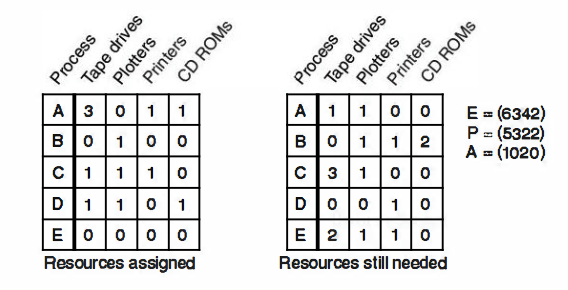
\includegraphics[width=0.6\textwidth]{images/bankers-multiple.png}
\end{center}


\end{frame}

\begin{frame}
\frametitle{Checking if a State is Safe}

\begin{enumerate}
	\item Look for a row in the matrix, $r$, where the unmet resource needs are less than or equal to the available resources in $A$.\\
	\quad If no such row exists, the system state is unsafe.
	\item Assume the process from $r$ gets all the resources it needs. Mark that process as terminated and put all its resources into $A$, the available pool.
	\item Repeat steps 1 and 2 until either:\\
	\quad (i) all processes are marked terminated and the initial state was safe; or \\
	\quad (ii) no process remains whose needs can be met; initial state is unsafe.
\end{enumerate}

If more than one process may be chosen in step 1, it does not matter which.

The pool of available resources will either stay the same or get larger.

\end{frame}

\begin{frame}
\frametitle{The Banker's Algorithm}

Determine if granting a resource makes the system unsafe: what-if calculation. 

Assume the resource granted; do the safe state calculation given that new state. 

If the result is that the state is unsafe, the request should be deferred or denied.

\end{frame}

\begin{frame}
\frametitle{The Banker's Algorithm: Useless?}

As great as the banker's algorithm is in theory, in practice it is utterly useless.

Processes rarely know in advance what their maximum resource needs will be. 

The number of processes is not fixed, but varies with users' wishes.

Finally, a resource that was thought to be available can suddenly vanish. 

Thus in practice, the banker's algorithm can almost never be used.


\end{frame}

\begin{frame}
\frametitle{Summary of Avoidance}

Avoidance techniques may be useful in preventing a deadlock from occurring without having to preempt resources or forbidding hold-and-wait conditions. 

Unfortunately, it requires a fixed number of known resources to allocate.

It also requires foreknowledge about what resources a process might need. 

Finally, because it deals with the worst case, it reduces system performance in the name of safety.

\end{frame}

\begin{frame}
\frametitle{Other Recommendations}

The avoidance techniques discussed previously require perfect information (or accurate worst-case guesses) about all the resources a process will ever need. 

In a world where this information is not known, thus far, all we have managed is to make deadlock less likely. 

\end{frame}

\begin{frame}
\frametitle{Deadlock Avoidance Recommendations: 1}
Minimize the number of critical sections and their length.

Mutual exclusion should be applied only where it is needed and to the minimal number of program statements.

\end{frame}

\begin{frame}
\frametitle{Deadlock Avoidance Recommendations: 2}

All tasks must release semaphores and resources as soon as possible.

This is not just polite, but also makes it less likely that processes are stuck waiting for one another.

\end{frame}

\begin{frame}
\frametitle{Deadlock Avoidance Recommendations: 3}

Do not suspend tasks when in the critical region. Avoid calling yield or some other call known to block.

\end{frame}

\begin{frame}
\frametitle{Deadlock Avoidance Recommendations: 4}

All critical regions must be error-free. 

This is obviously a desirable property for the whole program, but in critical region we must be especially careful.

\end{frame}

\begin{frame}
\frametitle{Deadlock Avoidance Recommendations: 5}

Do not allocate resources in interrupt handlers. 

Any resource allocation might block, and if an interrupt handler gets blocked, the whole system can be stuck.

\end{frame}

\begin{frame}
\frametitle{Deadlock Avoidance Recommendations: 6}

Always perform validity checks on pointers (or null checks) in critical regions. 

A segmentation fault or exception in the critical region can also mean never releasing the lock.

\end{frame}


\end{document}

